\begin{spacing}{1.5}
\chapter{\MakeUppercase{Technical Specification}}


% -----------------------------
% Table 3.1

% -----------------------------
\section{Requirements}
\subsection{Hardware Requirements}
\begin{itemize}
    \item System Type: Laptop/Desktop

\item Processor: Intel i5 / AMD Ryzen 5 or higher

\item RAM: Minimum 8 GB (Recommended: 16 GB for faster processing)

\item Storage: Minimum 10–20 GB free disk space (for dataset + models)

\item GPU (Optional): Not required, but useful for faster computation

\item Internet Connection: Required for dataset download and library installation
\end{itemize}
\subsection{Software Requirements}
\begin{itemize}
    \item Operating System: Windows / macOS / Linux

\item Programming Language: Python (Version 3.10 / 3.11)

\item Development Environment: Visual Studio Code (VS Code) / Jupyter Notebook


\item Version Control: Git/GitHub

\item Python Libraries:
\begin{itemize}
    \item pandas – for data manipulation

\item numpy – for numerical computations

\item scikit-learn – for machine learning models

\item matplotlib – for visualization

\item joblib – for saving/loading models

\item pyarrow – for handling parquet files

\item tqdm – for progress tracking
\end{itemize}

\item Dataset Source:OULAD dataset (UCI Machine Learning Repository)
\item Other Tools: Terminal / Command Prompt


\end{itemize}






\section{Feasibility Study}
\begin{itemize}
\item \textbf{Technical Feasibility}

\begin{itemize}
    \item Developed using Python and standard machine learning 
    \item libraries, with the use of resources which are readily available and easy to implement. 
\item The OULAD dataset is easily available online and ideal for processing. 
\item No specialized equipment is required—no need for GPUs. 
\item It works seamlessly on an average computer.
\end{itemize}
\item \textbf{Economic Feasibility}
\begin{itemize}
    \item The use of open-source software and libraries ensures that there are no licensing fees incurred.
\item No need to purchase any additional equipment. 
\item The process is economically viable.


\end{itemize}
\item \textbf{Operational Feasibility}
\begin{itemize}
    \item The process is user-friendly and adaptable for academic purposes. 
\item The results produced by the model include risk scores and predictions, making it easier for educators to make interventions.

\end{itemize}
\item \textbf{Time Feasibility}
\begin{itemize}
    \item The project is divided into stages: data collection, preprocessing, modeling, and evaluation

\item Each module can be completed within the given academic timeline

\item The overall system is feasible to implement within a semester
\end{itemize}
\item \textbf{Practical Feasibility}
\begin{itemize}
    \item Uses real-world dataset (OULAD), making results meaningful
\item Handles real challenges like missing data and behavioral variability

\item Can be extended into a full early warning system in the future

\end{itemize}




\end{itemize}




\section{System Specification}
The proposed system is designed to identify students at risk of academic burnout at an early stage using behavioral data from the OULAD dataset. It follows a structured machine learning workflow that converts raw student activity data into meaningful predictions.

\begin{itemize}
    \item \textbf{Input}

The model utilizes data obtained from students’ interactions within the OULAD database, including:

\begin{itemize}
    
\item Assignment marks and submission behavior
\item LMS interaction data, such as login and clickstream behavior
\item Course and engagement information







\end{itemize}
In terms of early detection, the model concentrates on using data from the beginning of the course, which could include the first four weeks.
\item \textbf{Processing}

The input data is first cleaned by handling missing or inconsistent values. It is then transformed into useful features that represent student behavior, such as:

\begin{itemize}
    \item Overall engagement level

\item Assignment completion rate

\item Activity consistency
\end{itemize}
These features help capture early signs of disengagement.

\item \textbf{Model}
\begin{itemize}
    \item Logistic Regression

\item Random Forest

\item Gradient Boosting

\item Support Vector Machine (SVM)
\end{itemize}
Each model is trained on the processed data and compared to determine performance.


\item \textbf{Output}


The system generates:
\begin{itemize}
    \item A burnout risk score (probability between 0 and 1).

\item A classification indicating whether a student is at risk or not.
\end{itemize}

Additionally, model performance is evaluated using metrics such as AUC-ROC, F1-score, and cross-validation.

\item \textbf{Storage}

The system stores:
\begin{itemize}
    \item Processed datasets in .parquet format

\item Trained models in .pkl format

\item Results and evaluation outputs in a reports folder
\end{itemize}





\end{itemize}
\section{Preparing your report/thesis/article using \LaTeX}
\paragraph{}
\subsection{Tables}
In the report, table can be defined in multiple ways according to the need.  For example, the latex code
{\scriptsize
\begin{verbatim}
\begin{table}[h!]
	\centering
	\caption{Country list}
	\renewcommand{\arraystretch}{1.3} % Row height
	\begin{tabular}{|l|l|l|l|}
		\hline
		\textbf{Country/Area Name} & \textbf{Description} & \textbf{ISO alpha 3 Code} & \textbf{ISO numeric Code} \\
		\hline
		Afghanistan & It is a Country & AFG & 004 \\
		Aland Islands & It is an Island & ALA & 248 \\
		Albania & It is a small city & ALB & 008 \\
		Algeria & It is a Country & DZA & 012 \\
		American Samoa & It is a Country & ASM & 016 \\
		\hline
	\end{tabular}
\end{table}
\end{verbatim}
}
defines the simple Table 3.1 in the document which is restricted to a single page.
\begin{table}[h!]
\centering
\caption{Country list}
\renewcommand{\arraystretch}{1.3} % Row height
\begin{tabular}{|l|l|l|l|}
\hline
\textbf{Country/Area Name} & \textbf{Description} & \textbf{ISO alpha 3 Code} & \textbf{ISO numeric Code} \\
\hline
Afghanistan & It is a Country & AFG & 004 \\
Aland Islands & It is an Island & ALA & 248 \\
Albania & It is a small city & ALB & 008 \\
Algeria & It is a Country & DZA & 012 \\
American Samoa & It is a Country & ASM & 016 \\
\hline
\end{tabular}
\end{table}

\pagebreak

The oversized table can be fit with in the page as follows: 
{\scriptsize
	\begin{verbatim}
		\begin{table}[h!]
			\centering
			\caption{Data units, sources, and dates}
			\renewcommand{\arraystretch}{1.3}
			\resizebox{\textwidth}{!}{
				\begin{tabular}{|l|l|l|l|}
					\hline
					\textbf{Variable} & \textbf{Dates} & \textbf{Units} & \textbf{Source} \\
					\hline
					Nominal Physical Capital Stock & 1950-1990 & Billions US\$ & Nehru and Dhareshwar (1993) \\
					Total Population & 1950-1990 & Billions & Nehru and Dhareshwar (1993) \\
					Nominal GDP & 1950-1990 & Billions US\$ & PWT \\
					Real GDP per capita & 1950-1990 & 2005 US\$ per capita & PWT \\
					\hline
			\end{tabular}}
		\end{table}
	\end{verbatim}
}
which produces the Table 3.2.

% -----------------------------
% Table 3.2
% -----------------------------
\begin{table}[h]
\centering
\caption{Data units, sources, and dates}
\renewcommand{\arraystretch}{1.3}
\resizebox{\textwidth}{!}{
\begin{tabular}{|l|l|l|l|}
\hline
\textbf{Variable} & \textbf{Dates} & \textbf{Units} & \textbf{Source} \\
\hline
Nominal Physical Capital Stock & 1950-1990 & Billions US\$ & Nehru and Dhareshwar (1993) \\
Total Population & 1950-1990 & Billions & Nehru and Dhareshwar (1993) \\
Nominal GDP & 1950-1990 & Billions US\$ & PWT \\
Real GDP per capita & 1950-1990 & 2005 US\$ per capita & PWT \\
\hline
\end{tabular}}
\end{table}

\paragraph{Defining the table span for more than one page}. 
The longtable (span for more than one page) can be achieved using following code. 
{\scriptsize
	\begin{verbatim}
		\begin{longtable}{|l|l|l|}
			\caption{This table can be used if more than one page table content is required. However it is limited to maximum of two pages only.} \label{tab:long} \\
			
			\hline \multicolumn{1}{|c|}{\textbf{First column}} & \multicolumn{1}{c|}{\textbf{Second column}} & \multicolumn{1}{c|}{\textbf{Third column}} \\ \hline 
			\endfirsthead
			
			\multicolumn{3}{c}%
			{{\bfseries \tablename\ \thetable{} -- continued from previous page}} \\
			\hline \multicolumn{1}{|c|}{\textbf{First column}} & \multicolumn{1}{c|}{\textbf{Second column}} & \multicolumn{1}{c|}{\textbf{Third column}} \\ \hline 
			\endhead
			
			\hline \multicolumn{3}{|r|}{{Continued on next page}} \\ \hline
			\endfoot
			
			\hline \hline
			\endlastfoot
			One & abcdef ghjijklmn & 123.456778 \\
			One & abcdef ghjijklmn & 123.456778 \\
			....
			....
			....
			One & abcdef ghjijklmn & 123.456778 \\
			One & abcdef ghjijklmn & 123.456778 \\
		\end{longtable}
	\end{verbatim}
}

\begin{longtable}{|l|l|l|}
	\caption{This table can be used if more than one page table content is required. However it is limited to maximum of two pages only.} \label{tab:long} \\
	
	\hline \multicolumn{1}{|c|}{\textbf{First column}} & \multicolumn{1}{c|}{\textbf{Second column}} & \multicolumn{1}{c|}{\textbf{Third column}} \\ \hline 
	\endfirsthead
	
	\multicolumn{3}{c}%
	{{\bfseries \tablename\ \thetable{} -- continued from previous page}} \\
	\hline \multicolumn{1}{|c|}{\textbf{First column}} & \multicolumn{1}{c|}{\textbf{Second column}} & \multicolumn{1}{c|}{\textbf{Third column}} \\ \hline 
	\endhead
	
	\hline \multicolumn{3}{|r|}{{Continued on next page}} \\ \hline
	\endfoot
	
	\hline \hline
	\endlastfoot
	
	One & abcdef ghjijklmn & 123.456778 \\
	One & abcdef ghjijklmn & 123.456778 \\
	One & abcdef ghjijklmn & 123.456778 \\
	One & abcdef ghjijklmn & 123.456778 \\
	One & abcdef ghjijklmn & 123.456778 \\
	One & abcdef ghjijklmn & 123.456778 \\
	One & abcdef ghjijklmn & 123.456778 \\
	One & abcdef ghjijklmn & 123.456778 \\
	One & abcdef ghjijklmn & 123.456778 \\
	One & abcdef ghjijklmn & 123.456778 \\
	One & abcdef ghjijklmn & 123.456778 \\
	One & abcdef ghjijklmn & 123.456778 \\
	One & abcdef ghjijklmn & 123.456778 \\
	One & abcdef ghjijklmn & 123.456778 \\
	One & abcdef ghjijklmn & 123.456778 \\
	One & abcdef ghjijklmn & 123.456778 \\
	One & abcdef ghjijklmn & 123.456778 \\
	One & abcdef ghjijklmn & 123.456778 \\
	One & abcdef ghjijklmn & 123.456778 \\
	One & abcdef ghjijklmn & 123.456778 \\
	One & abcdef ghjijklmn & 123.456778 \\
	One & abcdef ghjijklmn & 123.456778 \\
	One & abcdef ghjijklmn & 123.456778 \\
	One & abcdef ghjijklmn & 123.456778 \\
	One & abcdef ghjijklmn & 123.456778 \\
	One & abcdef ghjijklmn & 123.456778 \\
	One & abcdef ghjijklmn & 123.456778 \\
	One & abcdef ghjijklmn & 123.456778 \\
	One & abcdef ghjijklmn & 123.456778 \\
	One & abcdef ghjijklmn & 123.456778 \\
	One & abcdef ghjijklmn & 123.456778 \\
	One & abcdef ghjijklmn & 123.456778 \\
	One & abcdef ghjijklmn & 123.456778 \\
	One & abcdef ghjijklmn & 123.456778 \\
	One & abcdef ghjijklmn & 123.456778 \\
	One & abcdef ghjijklmn & 123.456778 \\
	One & abcdef ghjijklmn & 123.456778 \\
	One & abcdef ghjijklmn & 123.456778 \\
	One & abcdef ghjijklmn & 123.456778 \\
	One & abcdef ghjijklmn & 123.456778 \\
	One & abcdef ghjijklmn & 123.456778 \\
	One & abcdef ghjijklmn & 123.456778 \\
	One & abcdef ghjijklmn & 123.456778 \\
	One & abcdef ghjijklmn & 123.456778 \\
	One & abcdef ghjijklmn & 123.456778 \\
	One & abcdef ghjijklmn & 123.456778 \\
	One & abcdef ghjijklmn & 123.456778 \\
	One & abcdef ghjijklmn & 123.456778 \\
	One & abcdef ghjijklmn & 123.456778 \\
	One & abcdef ghjijklmn & 123.456778 \\
	One & abcdef ghjijklmn & 123.456778 \\
	One & abcdef ghjijklmn & 123.456778 \\
	One & abcdef ghjijklmn & 123.456778 \\
	One & abcdef ghjijklmn & 123.456778 \\
	One & abcdef ghjijklmn & 123.456778 \\
	One & abcdef ghjijklmn & 123.456778 \\
	One & abcdef ghjijklmn & 123.456778 \\
	One & abcdef ghjijklmn & 123.456778 \\
	One & abcdef ghjijklmn & 123.456778 \\
	One & abcdef ghjijklmn & 123.456778 \\
	One & abcdef ghjijklmn & 123.456778 \\
	One & abcdef ghjijklmn & 123.456778 \\
	One & abcdef ghjijklmn & 123.456778 \\
	One & abcdef ghjijklmn & 123.456778 \\
	One & abcdef ghjijklmn & 123.456778 \\
	One & abcdef ghjijklmn & 123.456778 \\
	One & abcdef ghjijklmn & 123.456778 \\
	One & abcdef ghjijklmn & 123.456778 \\
	One & abcdef ghjijklmn & 123.456778 \\
	One & abcdef ghjijklmn & 123.456778 \\
	One & abcdef ghjijklmn & 123.456778 \\
	One & abcdef ghjijklmn & 123.456778 \\
	One & abcdef ghjijklmn & 123.456778 \\
	One & abcdef ghjijklmn & 123.456778 \\
	One & abcdef ghjijklmn & 123.456778 \\
	One & abcdef ghjijklmn & 123.456778 \\
	One & abcdef ghjijklmn & 123.456778 \\
	One & abcdef ghjijklmn & 123.456778 \\
	One & abcdef ghjijklmn & 123.456778 \\
	One & abcdef ghjijklmn & 123.456778 \\
\end{longtable}

The table can also be presented in the Landscape orientation as follows: 
\begin{sidewaystable}
	\centering
	\caption{This is long table presented in Landscape orientation}
	\begin{tabular}{|c|c|c|c|c|c|c|c|c|c|c|c}
		\hline
		col 1 & col 2 & col 3 & col 4 & col 5 & col 6 & col 7 & col 8 & col 9 & col 10 & col 11 & col 12 \\
		One & abcdef ghjijklmn & 123.456778 & One & abcdef ghjijklmn & 123.456778 & One & abcdef ghjijklmn & 123.456778 & One & abcdef ghjijklmn &  123.456778 \\
		One & abcdef ghjijklmn & 123.456778 & One & abcdef ghjijklmn & 123.456778 & One & abcdef ghjijklmn & 123.456778 & One & abcdef ghjijklmn &  123.456778 \\
		One & abcdef ghjijklmn & 123.456778 & One & abcdef ghjijklmn & 123.456778 & One & abcdef ghjijklmn & 123.456778 & One & abcdef ghjijklmn &  123.456778 \\
		One & abcdef ghjijklmn & 123.456778 & One & abcdef ghjijklmn & 123.456778 & One & abcdef ghjijklmn & 123.456778 & One & abcdef ghjijklmn &  123.456778 \\
		\hline
	\end{tabular}
\end{sidewaystable}	


\subsection{Equations}
In line equation can be defined in latex as \verb|$\hat{y} = f(x; W, b)$|. This code produce the formula as $\hat{y} = f(x; W, b)$ . 

\paragraph{Equations}
In latex, the equation can be defined using following commands: 
\begin{verbatim}
	\begin{equation}
		\delta^{L} = \frac{\partial \mathcal{L}}{\partial a^{L}} \odot \sigma'(z^{L})
	\end{equation}
\end{verbatim}
which will produce the Equation 3.1. You can use \verb|$\delta^{L}$| to represent $\delta^{L}$ in the running text.  For example, $\odot$ is a Hadamard operator. 
\begin{equation}
	\delta^{L} = \frac{\partial \mathcal{L}}{\partial a^{L}} \odot \sigma'(z^{L})
\end{equation}

\subsection{Figures}
\paragraph{Figure} Figures can be included in the latex document. One simple figure/image can be included as 
\begin{verbatim}
	\begin{figure}[h]
		\centering
		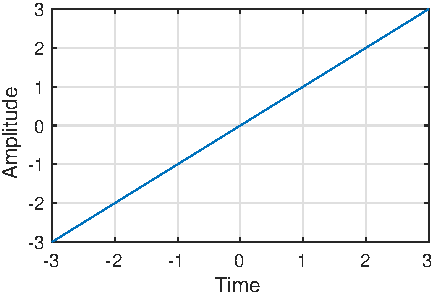
\includegraphics[width=0.5\linewidth]{images/sample-graph.pdf}
		\caption{Sample Diagram}
		\label{fig:universe}
	\end{figure}
\end{verbatim} 
which will produce the output as 
\begin{figure}[!h]
	\centering
	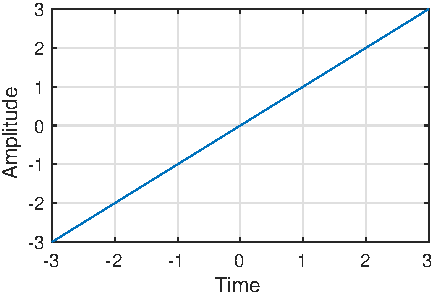
\includegraphics[width=0.5\linewidth]{images/sample-graph.pdf}
	\caption{Sample Diagram}
	\label{fig:universe1}
\end{figure}
\linebreak
More than one figures can be shown adjacent using following code
\begin{verbatim}
	\begin{figure}[h!]
		\centering
		% Left image (a)
		\begin{subfigure}[b]{0.45\linewidth}
			\centering
			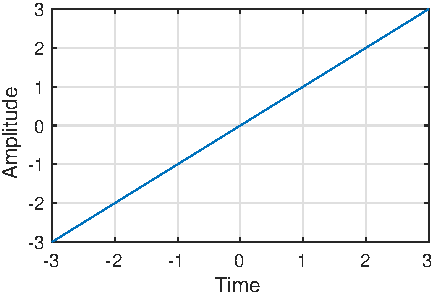
\includegraphics[width=\textwidth]{images/sample-graph.pdf} % replace with your image filename
			\caption{Example Graph}
			\label{fig:fruitsA}
		\end{subfigure}
		\hfill
		% Right image (b)
		\begin{subfigure}[b]{0.45\linewidth}
			\centering
			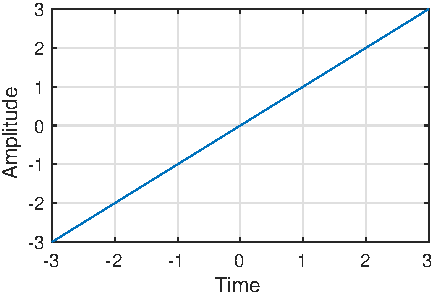
\includegraphics[width=\textwidth]{images/sample-graph.pdf} % replace with your image filename
			\caption{Example Graph}
			\label{fig:fruitsC}
		\end{subfigure}
		
		\caption{Commonly available fruits}
		\label{fig:common_fruits}
	\end{figure}
\end{verbatim}
The above code will produce the results as 
\begin{figure}[h!]
	\centering
	% Left image (a)
	\begin{subfigure}[b]{0.45\linewidth}
		\centering
		\rotatebox{45}{
		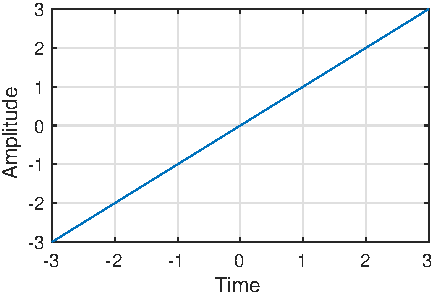
\includegraphics[width=\textwidth]{images/sample-graph.pdf} %	 replace with your image filename
		}
		
	
		\label{fig:fruitsAA}
	\end{subfigure}
	\hfill
	% Right image (b)
	\begin{subfigure}[b]{0.45\linewidth}
		\centering
		\rotatebox{-45}{
		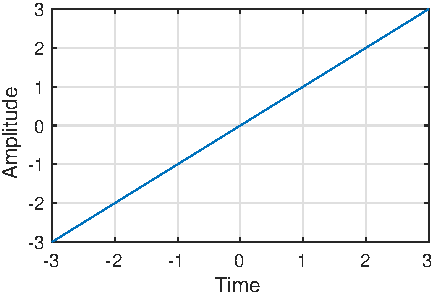
\includegraphics[width=\textwidth]{images/sample-graph.pdf} % replace with your image filename
		}
		\label{fig:fruitsCC}
	\end{subfigure}
	
	\caption{Figures with rotation}
	\label{fig:common_fruitsA}
\end{figure}

\subsection{Pseudo code / Algorithm}
The algorithm or pseudo code can be added using following code
\begin{verbatim}
	\begin{algorithm}
		\caption{An example algorithm with caption}\label{alg:cap}
		\begin{algorithmic}
			\Require $n \geq 0$
			\Ensure $y = x^n$
			\State $y \gets 1$
			\State $X \gets x$
			\State $N \gets n$
			\While{$N \neq 0$}
			\If{$N$ is even}
			\State $X \gets X \times X$
			\State $N \gets \frac{N}{2}$  \Comment{This is a comment}
			\ElsIf{$N$ is odd}
			\State $y \gets y \times X$
			\State $N \gets N - 1$
			\EndIf
			\EndWhile
		\end{algorithmic}
	\end{algorithm}
\end{verbatim}
This code will produce the following output in the report.
\begin{algorithm}
	\caption{An example algorithm with caption}\label{alg:cap}
	\begin{algorithmic}
		\Require $n \geq 0$
		\Ensure $y = x^n$
		\State $y \gets 1$
		\State $X \gets x$
		\State $N \gets n$
		\While{$N \neq 0$}
		\If{$N$ is even}
		\State $X \gets X \times X$
		\State $N \gets \frac{N}{2}$  \Comment{This is a comment}
		\ElsIf{$N$ is odd}
		\State $y \gets y \times X$
		\State $N \gets N - 1$
		\EndIf
		\EndWhile
	\end{algorithmic}
\end{algorithm}
\end{spacing}